\chapter*{\textbf{Эксперимент №2: Сравнение эффективности ссылочных и векторных структур}}
\addcontentsline{toc}{chapter}{Эксперимент №2: Сравнение эффективности ссылочных и векторных структур}

\subsection*{\textbf{Цель эксперимента}}
Оценка влияния зависимости команд по данным на эффективность вычислений. 

\subsection*{\textbf{Описание проблемы}}
Обработка зависимых данных происходит в тех случаях, когда результат работы одной команды используется в качестве адреса операнда другой. При программировании на языках высокого уровня такими операндами являются указатели, активно используемые при обработке ссылочных структур данных: списков, деревьев, графов. Обработка данных структур процессорами с длинными конвейерами команд приводит к заметному увеличению времени работы алгоритмов: адрес загружаемого операнда становится известным только после обработки предыдущей команды. В противоположность этому, обработка векторных структур, таких как массивы, позволяет эффективно использовать аппаратные возможности ЭВМ. 

\textbf{\subsection*{\textbf{Результаты эксперимента}}}
На рисунке \ref{img:experiment_2} представлен график, полученный в результате эксперимента с исходными параметрами:
\begin{itemize}
	\item количество элементов в списке (М) = 1;
	\item максимальная фрагментации списка (К) = 32;
	\item шаг увеличения фрагментации (К) = 1.
\end{itemize}

\begin{figure}[H]
	\centering{
		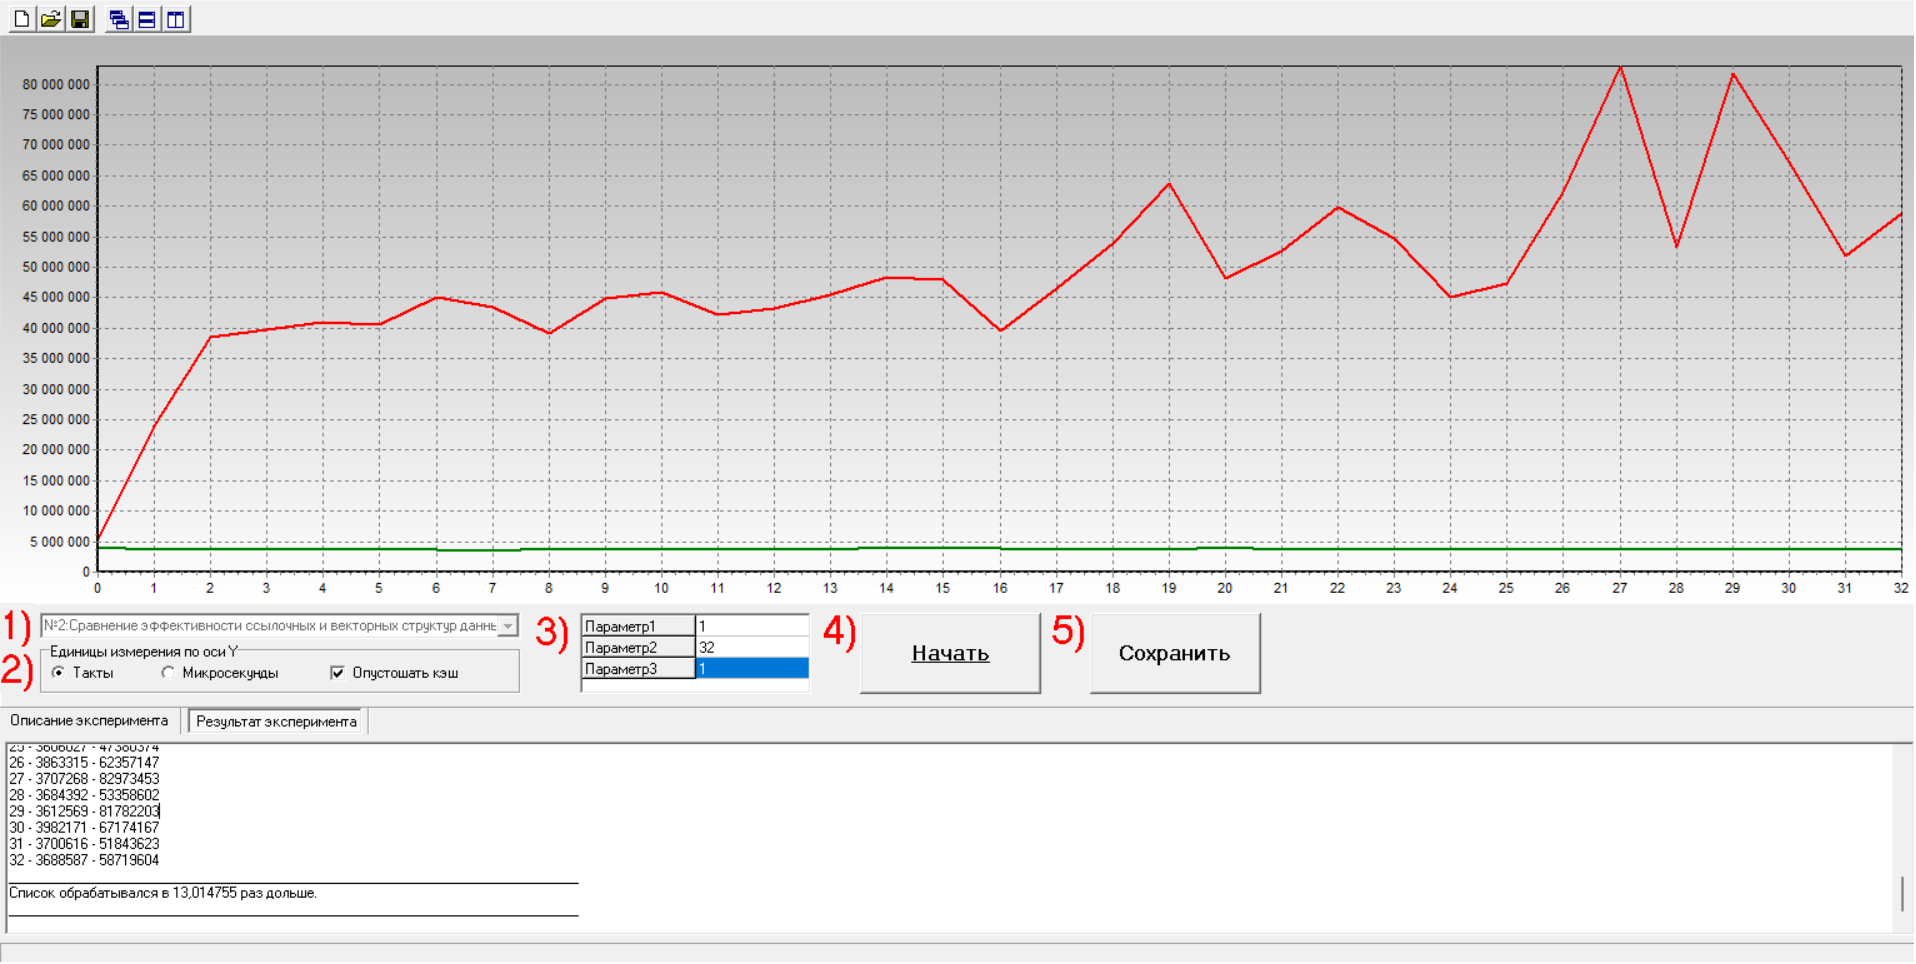
\includegraphics[scale=0.4]{images/experiment_2_1}
		\caption{Эксперимент №2}
		\label{img:experiment_2}
	}
\end{figure}

Результат сравнения времени (как вывод программы) представлен на рисунке \ref{img:experiment_2}. Как видно на рисунке, список обрабатывается в 13 раз медленнее. 

\subsection*{\textbf{Вывод}}
Использовать структуры данных надо с учетом технологического фактора определенной задачи. Если решаемая задача предполагает возможность использования массива, то надо использовать его, особенно если использование списка не дает существенной разницы (особенно выигрыша во времени).